\section{Demonstration Setup}
The screenshots in this chapter were taken from the live Windows application running on the development laptop. The default webcam was used. The user sat at a desk, faced the camera, and held one hand inside the frame. Lighting was ordinary indoor room light. No cloud service was used during the demonstration.

\section{Hand Detection}
Figure~\ref{fig:hand} shows the tracker overlay. The skeleton follows the twenty-one MediaPipe landmarks, and the window remains a mirrored selfie view. This is the first check in a viva: if the skeleton does not sit on the hand, later classification cannot be trusted.

\begin{figure}[H]
\centering
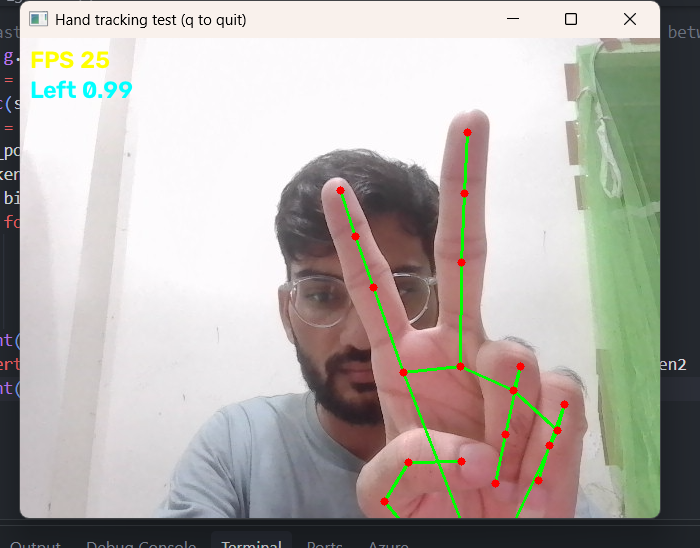
\includegraphics[width=0.72\textwidth]{Hand_detection.png}
\caption{Live hand detection with MediaPipe landmark overlay}
\label{fig:hand}
\end{figure}

\section{Gesture to Text}
Figure~\ref{fig:sign} shows a recognised pose converted into on-screen text. After the hand is held steady, the overlay stops saying ``Checking...'' and shows the confirmed word. The same word is queued for speech. Diagnostic text on the window reports the corrected hand side, the finger bit pattern and the pointing orientation. Those fields are useful while explaining the classifier in a viva, because they show why a particular table entry was chosen.

\begin{figure}[H]
\centering
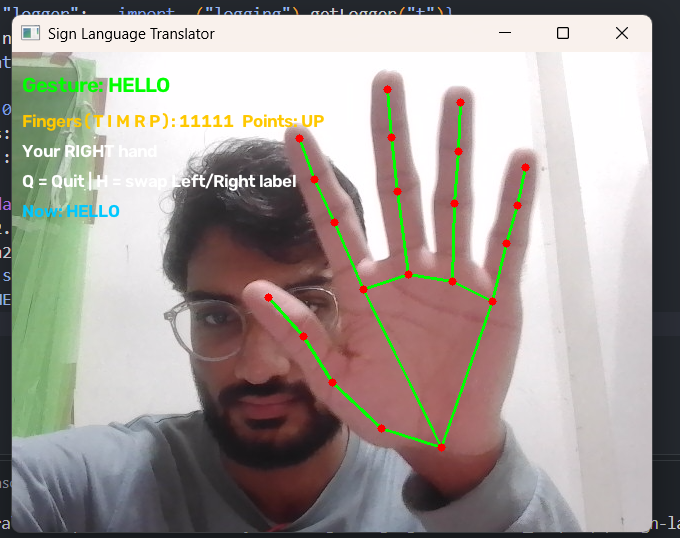
\includegraphics[width=0.72\textwidth]{sign_language.png}
\caption{Recognised gesture shown as text on the live window}
\label{fig:sign}
\end{figure}

\section{No Hand State}
Figure~\ref{fig:nohand} shows the empty-frame behaviour. When the hand leaves the camera, the overlay returns to ``No hand detected''. After about 0.15 seconds the speech controller stops the current utterance and drops pending words. This is an important result for a live demo. Without it, the last spoken word would keep playing after the user has already put the hand down.

\begin{figure}[H]
\centering
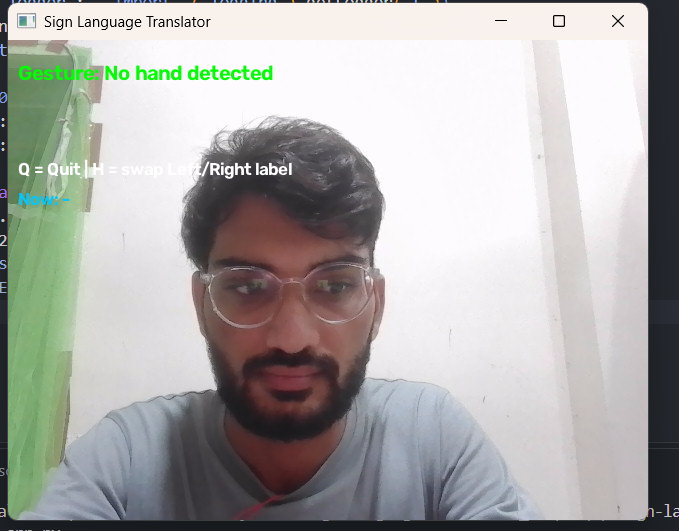
\includegraphics[width=0.72\textwidth]{when_no_hand.png}
\caption{Application state when no hand is visible}
\label{fig:nohand}
\end{figure}

\section{Large Vocabulary}
Figure~\ref{fig:more} shows that the system is not limited to a handful of named signs. More than five hundred everyday gestures were added for this project. The extra words cover greetings, family, school, food, travel, numbers, colours and common actions. In the demonstration, changing from one stable pose to another updates the overlay and interrupts the previous speech so the new word is heard without waiting.

\begin{figure}[H]
\centering
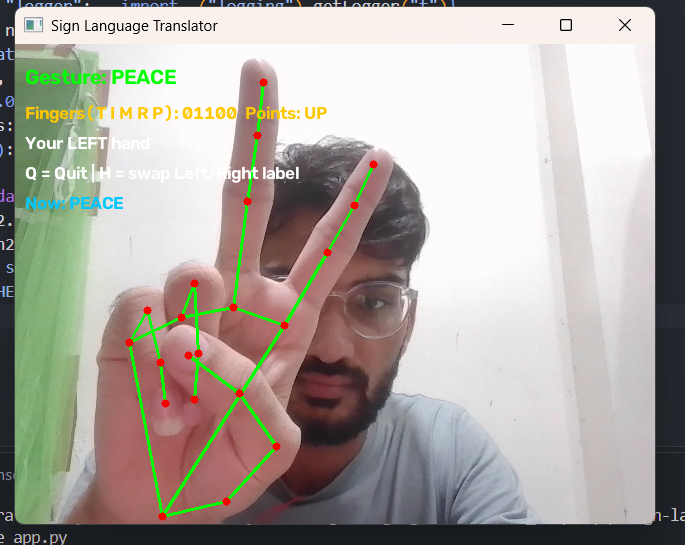
\includegraphics[width=0.72\textwidth]{more_gestures.png}
\caption{Live recognition from the 500+ gesture vocabulary}
\label{fig:more}
\end{figure}

\section{Synthetic Tests}
Webcam-free tests in \code{tests/test_gestures.py} build synthetic landmarks for finger patterns and orientations. Named poses such as HELLO, I LOVE YOU, YES, PEACE and FIST return the expected labels. Thumbs-down is recognised as NO. Left and right hands produce different table entries for the same finger pattern after handedness correction. Aspect-ratio correction is checked so that a stretched frame does not change the label. A short hold-to-confirm sequence is also simulated by feeding GestureState at thirty updates per second.

Under a synthetic noise protocol, filtered YES and HELLO labels remained above ninety percent, and a five-pose burst was spoken in the expected order. These numbers describe the synthetic protocol, not a human sign-language benchmark. They are reported here because they document anti-flicker behaviour without claiming ASL or ISL accuracy.

\section{Observed Runtime Behaviour}
On the development laptop the camera loop stayed interactive while speech was playing. Changing pose while a word was still being spoken cut off the old audio. Holding the same pose did not repeat the word. Removing the hand silenced the speakers. Those observations match the design of the generation counter in \code{SpeechController}. Frame rate was not formally benchmarked against ONNX in this stage. Qualitatively, tracking and overlay remained usable for a live viva on CPU.
